% Options for packages loaded elsewhere
\PassOptionsToPackage{unicode}{hyperref}
\PassOptionsToPackage{hyphens}{url}
\PassOptionsToPackage{dvipsnames,svgnames,x11names}{xcolor}
%
\documentclass[
  letterpaper,
  DIV=11,
  numbers=noendperiod]{scrartcl}

\usepackage{amsmath,amssymb}
\usepackage{iftex}
\ifPDFTeX
  \usepackage[T1]{fontenc}
  \usepackage[utf8]{inputenc}
  \usepackage{textcomp} % provide euro and other symbols
\else % if luatex or xetex
  \usepackage{unicode-math}
  \defaultfontfeatures{Scale=MatchLowercase}
  \defaultfontfeatures[\rmfamily]{Ligatures=TeX,Scale=1}
\fi
\usepackage{lmodern}
\ifPDFTeX\else  
    % xetex/luatex font selection
\fi
% Use upquote if available, for straight quotes in verbatim environments
\IfFileExists{upquote.sty}{\usepackage{upquote}}{}
\IfFileExists{microtype.sty}{% use microtype if available
  \usepackage[]{microtype}
  \UseMicrotypeSet[protrusion]{basicmath} % disable protrusion for tt fonts
}{}
\makeatletter
\@ifundefined{KOMAClassName}{% if non-KOMA class
  \IfFileExists{parskip.sty}{%
    \usepackage{parskip}
  }{% else
    \setlength{\parindent}{0pt}
    \setlength{\parskip}{6pt plus 2pt minus 1pt}}
}{% if KOMA class
  \KOMAoptions{parskip=half}}
\makeatother
\usepackage{xcolor}
\setlength{\emergencystretch}{3em} % prevent overfull lines
\setcounter{secnumdepth}{-\maxdimen} % remove section numbering
% Make \paragraph and \subparagraph free-standing
\ifx\paragraph\undefined\else
  \let\oldparagraph\paragraph
  \renewcommand{\paragraph}[1]{\oldparagraph{#1}\mbox{}}
\fi
\ifx\subparagraph\undefined\else
  \let\oldsubparagraph\subparagraph
  \renewcommand{\subparagraph}[1]{\oldsubparagraph{#1}\mbox{}}
\fi

\usepackage{color}
\usepackage{fancyvrb}
\newcommand{\VerbBar}{|}
\newcommand{\VERB}{\Verb[commandchars=\\\{\}]}
\DefineVerbatimEnvironment{Highlighting}{Verbatim}{commandchars=\\\{\}}
% Add ',fontsize=\small' for more characters per line
\usepackage{framed}
\definecolor{shadecolor}{RGB}{241,243,245}
\newenvironment{Shaded}{\begin{snugshade}}{\end{snugshade}}
\newcommand{\AlertTok}[1]{\textcolor[rgb]{0.68,0.00,0.00}{#1}}
\newcommand{\AnnotationTok}[1]{\textcolor[rgb]{0.37,0.37,0.37}{#1}}
\newcommand{\AttributeTok}[1]{\textcolor[rgb]{0.40,0.45,0.13}{#1}}
\newcommand{\BaseNTok}[1]{\textcolor[rgb]{0.68,0.00,0.00}{#1}}
\newcommand{\BuiltInTok}[1]{\textcolor[rgb]{0.00,0.23,0.31}{#1}}
\newcommand{\CharTok}[1]{\textcolor[rgb]{0.13,0.47,0.30}{#1}}
\newcommand{\CommentTok}[1]{\textcolor[rgb]{0.37,0.37,0.37}{#1}}
\newcommand{\CommentVarTok}[1]{\textcolor[rgb]{0.37,0.37,0.37}{\textit{#1}}}
\newcommand{\ConstantTok}[1]{\textcolor[rgb]{0.56,0.35,0.01}{#1}}
\newcommand{\ControlFlowTok}[1]{\textcolor[rgb]{0.00,0.23,0.31}{#1}}
\newcommand{\DataTypeTok}[1]{\textcolor[rgb]{0.68,0.00,0.00}{#1}}
\newcommand{\DecValTok}[1]{\textcolor[rgb]{0.68,0.00,0.00}{#1}}
\newcommand{\DocumentationTok}[1]{\textcolor[rgb]{0.37,0.37,0.37}{\textit{#1}}}
\newcommand{\ErrorTok}[1]{\textcolor[rgb]{0.68,0.00,0.00}{#1}}
\newcommand{\ExtensionTok}[1]{\textcolor[rgb]{0.00,0.23,0.31}{#1}}
\newcommand{\FloatTok}[1]{\textcolor[rgb]{0.68,0.00,0.00}{#1}}
\newcommand{\FunctionTok}[1]{\textcolor[rgb]{0.28,0.35,0.67}{#1}}
\newcommand{\ImportTok}[1]{\textcolor[rgb]{0.00,0.46,0.62}{#1}}
\newcommand{\InformationTok}[1]{\textcolor[rgb]{0.37,0.37,0.37}{#1}}
\newcommand{\KeywordTok}[1]{\textcolor[rgb]{0.00,0.23,0.31}{#1}}
\newcommand{\NormalTok}[1]{\textcolor[rgb]{0.00,0.23,0.31}{#1}}
\newcommand{\OperatorTok}[1]{\textcolor[rgb]{0.37,0.37,0.37}{#1}}
\newcommand{\OtherTok}[1]{\textcolor[rgb]{0.00,0.23,0.31}{#1}}
\newcommand{\PreprocessorTok}[1]{\textcolor[rgb]{0.68,0.00,0.00}{#1}}
\newcommand{\RegionMarkerTok}[1]{\textcolor[rgb]{0.00,0.23,0.31}{#1}}
\newcommand{\SpecialCharTok}[1]{\textcolor[rgb]{0.37,0.37,0.37}{#1}}
\newcommand{\SpecialStringTok}[1]{\textcolor[rgb]{0.13,0.47,0.30}{#1}}
\newcommand{\StringTok}[1]{\textcolor[rgb]{0.13,0.47,0.30}{#1}}
\newcommand{\VariableTok}[1]{\textcolor[rgb]{0.07,0.07,0.07}{#1}}
\newcommand{\VerbatimStringTok}[1]{\textcolor[rgb]{0.13,0.47,0.30}{#1}}
\newcommand{\WarningTok}[1]{\textcolor[rgb]{0.37,0.37,0.37}{\textit{#1}}}

\providecommand{\tightlist}{%
  \setlength{\itemsep}{0pt}\setlength{\parskip}{0pt}}\usepackage{longtable,booktabs,array}
\usepackage{calc} % for calculating minipage widths
% Correct order of tables after \paragraph or \subparagraph
\usepackage{etoolbox}
\makeatletter
\patchcmd\longtable{\par}{\if@noskipsec\mbox{}\fi\par}{}{}
\makeatother
% Allow footnotes in longtable head/foot
\IfFileExists{footnotehyper.sty}{\usepackage{footnotehyper}}{\usepackage{footnote}}
\makesavenoteenv{longtable}
\usepackage{graphicx}
\makeatletter
\def\maxwidth{\ifdim\Gin@nat@width>\linewidth\linewidth\else\Gin@nat@width\fi}
\def\maxheight{\ifdim\Gin@nat@height>\textheight\textheight\else\Gin@nat@height\fi}
\makeatother
% Scale images if necessary, so that they will not overflow the page
% margins by default, and it is still possible to overwrite the defaults
% using explicit options in \includegraphics[width, height, ...]{}
\setkeys{Gin}{width=\maxwidth,height=\maxheight,keepaspectratio}
% Set default figure placement to htbp
\makeatletter
\def\fps@figure{htbp}
\makeatother

\KOMAoption{captions}{tableheading}
\makeatletter
\makeatother
\makeatletter
\makeatother
\makeatletter
\@ifpackageloaded{caption}{}{\usepackage{caption}}
\AtBeginDocument{%
\ifdefined\contentsname
  \renewcommand*\contentsname{Table of contents}
\else
  \newcommand\contentsname{Table of contents}
\fi
\ifdefined\listfigurename
  \renewcommand*\listfigurename{List of Figures}
\else
  \newcommand\listfigurename{List of Figures}
\fi
\ifdefined\listtablename
  \renewcommand*\listtablename{List of Tables}
\else
  \newcommand\listtablename{List of Tables}
\fi
\ifdefined\figurename
  \renewcommand*\figurename{Figure}
\else
  \newcommand\figurename{Figure}
\fi
\ifdefined\tablename
  \renewcommand*\tablename{Table}
\else
  \newcommand\tablename{Table}
\fi
}
\@ifpackageloaded{float}{}{\usepackage{float}}
\floatstyle{ruled}
\@ifundefined{c@chapter}{\newfloat{codelisting}{h}{lop}}{\newfloat{codelisting}{h}{lop}[chapter]}
\floatname{codelisting}{Listing}
\newcommand*\listoflistings{\listof{codelisting}{List of Listings}}
\makeatother
\makeatletter
\@ifpackageloaded{caption}{}{\usepackage{caption}}
\@ifpackageloaded{subcaption}{}{\usepackage{subcaption}}
\makeatother
\makeatletter
\@ifpackageloaded{tcolorbox}{}{\usepackage[skins,breakable]{tcolorbox}}
\makeatother
\makeatletter
\@ifundefined{shadecolor}{\definecolor{shadecolor}{rgb}{.97, .97, .97}}
\makeatother
\makeatletter
\makeatother
\makeatletter
\makeatother
\ifLuaTeX
  \usepackage{selnolig}  % disable illegal ligatures
\fi
\IfFileExists{bookmark.sty}{\usepackage{bookmark}}{\usepackage{hyperref}}
\IfFileExists{xurl.sty}{\usepackage{xurl}}{} % add URL line breaks if available
\urlstyle{same} % disable monospaced font for URLs
\hypersetup{
  pdftitle={Vapour Sensing System for Transistor Biosensing},
  colorlinks=true,
  linkcolor={blue},
  filecolor={Maroon},
  citecolor={Blue},
  urlcolor={Blue},
  pdfcreator={LaTeX via pandoc}}

\title{Vapour Sensing System for Transistor Biosensing}
\author{}
\date{}

\begin{document}
\maketitle
\ifdefined\Shaded\renewenvironment{Shaded}{\begin{tcolorbox}[borderline west={3pt}{0pt}{shadecolor}, boxrule=0pt, interior hidden, frame hidden, enhanced, breakable, sharp corners]}{\end{tcolorbox}}\fi

\begin{Shaded}
\begin{Highlighting}[]
\ImportTok{import}\NormalTok{ re}

\CommentTok{\# Dictionary to map month abbreviations to numbers}
\NormalTok{month\_mapping }\OperatorTok{=}\NormalTok{ \{}
    \StringTok{"jan"}\NormalTok{: }\StringTok{"1"}\NormalTok{,}
    \StringTok{"feb"}\NormalTok{: }\StringTok{"2"}\NormalTok{,}
    \StringTok{"mar"}\NormalTok{: }\StringTok{"3"}\NormalTok{,}
    \StringTok{"apr"}\NormalTok{: }\StringTok{"4"}\NormalTok{,}
    \StringTok{"may"}\NormalTok{: }\StringTok{"5"}\NormalTok{,}
    \StringTok{"jun"}\NormalTok{: }\StringTok{"6"}\NormalTok{,}
    \StringTok{"jul"}\NormalTok{: }\StringTok{"7"}\NormalTok{,}
    \StringTok{"aug"}\NormalTok{: }\StringTok{"8"}\NormalTok{,}
    \StringTok{"sep"}\NormalTok{: }\StringTok{"9"}\NormalTok{,}
    \StringTok{"oct"}\NormalTok{: }\StringTok{"10"}\NormalTok{,}
    \StringTok{"nov"}\NormalTok{: }\StringTok{"11"}\NormalTok{,}
    \StringTok{"dec"}\NormalTok{: }\StringTok{"12"}
\NormalTok{\}}

\CommentTok{\# Read the content of the original .bib file with UTF{-}8 encoding}
\ControlFlowTok{with} \BuiltInTok{open}\NormalTok{(}\StringTok{"references.bib"}\NormalTok{, }\StringTok{"r"}\NormalTok{, encoding}\OperatorTok{=}\StringTok{"utf{-}8"}\NormalTok{) }\ImportTok{as} \BuiltInTok{file}\NormalTok{:}
\NormalTok{    bib\_content }\OperatorTok{=} \BuiltInTok{file}\NormalTok{.read()}

\CommentTok{\# Replace month abbreviations with numbers using a single regex}
\NormalTok{pattern\_month }\OperatorTok{=} \VerbatimStringTok{r\textquotesingle{}month\textbackslash{}s*=\textbackslash{}s*\{([a{-}z]+)\},\textquotesingle{}}
\KeywordTok{def}\NormalTok{ replace\_month(match):}
\NormalTok{    month\_abbrev }\OperatorTok{=}\NormalTok{ match.group(}\DecValTok{1}\NormalTok{)}
\NormalTok{    month\_number }\OperatorTok{=}\NormalTok{ month\_mapping.get(month\_abbrev, month\_abbrev)}
    \ControlFlowTok{return} \SpecialStringTok{f\textquotesingle{}month = }\CharTok{\{\{}\SpecialCharTok{\{}\NormalTok{month\_number}\SpecialCharTok{\}}\CharTok{\}\}}\SpecialStringTok{,\textquotesingle{}}

\NormalTok{modified\_content }\OperatorTok{=}\NormalTok{ re.sub(pattern\_month, replace\_month, bib\_content, flags}\OperatorTok{=}\NormalTok{re.IGNORECASE)}

\CommentTok{\# Replace "\%" with "\textbackslash{}\%" when not preceded by a backslash}
\NormalTok{modified\_content }\OperatorTok{=}\NormalTok{ re.sub(}\VerbatimStringTok{r\textquotesingle{}(?\textless{}!\textbackslash{}\textbackslash{})\%\textquotesingle{}}\NormalTok{, }\VerbatimStringTok{r\textquotesingle{}\textbackslash{}\textbackslash{}\%\textquotesingle{}}\NormalTok{, modified\_content)}

\CommentTok{\# Write the modified content back to the original .bib file with UTF{-}8 encoding}
\ControlFlowTok{with} \BuiltInTok{open}\NormalTok{(}\StringTok{"references.bib"}\NormalTok{, }\StringTok{"w"}\NormalTok{, encoding}\OperatorTok{=}\StringTok{"utf{-}8"}\NormalTok{) }\ImportTok{as} \BuiltInTok{file}\NormalTok{:}
    \BuiltInTok{file}\NormalTok{.write(modified\_content)}
\end{Highlighting}
\end{Shaded}

\hypertarget{general-remarks}{%
\subsection{General Remarks}\label{general-remarks}}

\hypertarget{technical-notes}{%
\subsection{Technical Notes}\label{technical-notes}}

\hypertarget{delivery-system}{%
\subsubsection{Delivery System}\label{delivery-system}}

\hypertarget{control-system}{%
\subsubsection{Control System}\label{control-system}}

\hypertarget{electronics}{%
\paragraph*{Electronics}\label{electronics}}
\addcontentsline{toc}{paragraph}{Electronics}

\hypertarget{software}{%
\paragraph*{Software}\label{software}}
\addcontentsline{toc}{paragraph}{Software}

Two LabView Virtual Instruments (VIs) were adapted from pre-existing VIs
for operating the mass flow controllers and monitoring vapour flow into
the device chamber, as well as monitoring temperature and humidity in
the vapour delivery system's manifold. These VIs were named ``\,'' A
third VI was developed in parallel which combined the first two Virtual
Instruments, alongside allowing the sequence of values to control the
mass flow controllers.

From Honours report: ``\,``\,'' Figure 12 gives the right side of the
front panel of the LabView VI sample with vapour.VI, which letsus preset
an autonomously-performed vapour sensing sequence. Each row in each
array module corresponds to a differennest step in this sequence. The
`howManySteps' module lets us set how many of these steps are performed.
The `Durations Array' module determines the length of time in seconds
each step is performed over. The `Carrier Flows Array' and `Dilution
Flows Array' modules let us set the carrier flow and dilution flow,
respectively, in standard cubic centimetres per minute (sccm) through
the gas rig at each step. The carrier flow pushes analyte vapour into
the vapour-sensing device chamber, while dilution flow is used to modify
the flow behaviour of the analyte vapour entering the chamber. The
vapour sensing sequence as depicted in Figure 12 was used for all vapour
sensing runs in this investigation. At the end of the sequence, the data
collected about the vapour sensing process was saved as an .lvm file.
``\,``\,''

\hypertarget{design}{%
\subsection{Design}\label{design}}

\hypertarget{original-layout}{%
\subsubsection{Original Layout}\label{original-layout}}

\begin{figure}

{\centering 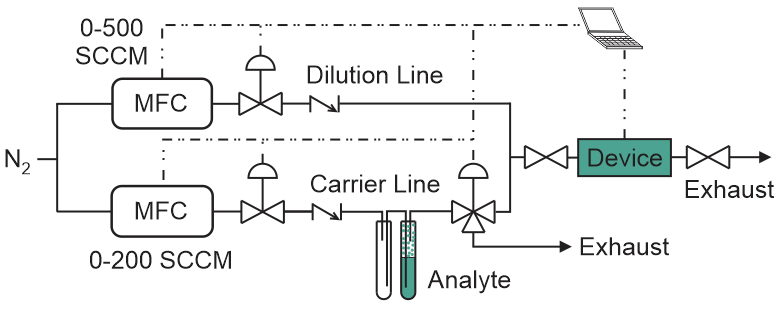
\includegraphics[width=0.9\textwidth,height=\textheight]{figures/ch5/PID_V0.png}

}

\caption{Vapour Delivery System - P\&ID of Existing System}

\end{figure}

\hypertarget{stage-i-design}{%
\subsubsection{Stage I Design}\label{stage-i-design}}

\hypertarget{stage-ii-design}{%
\subsubsection{Stage II Design}\label{stage-ii-design}}

\hypertarget{future-improvements}{%
\subsubsection{Future Improvements}\label{future-improvements}}

\hypertarget{validating-vapour-delivery-system}{%
\subsection{Validating Vapour Delivery
System}\label{validating-vapour-delivery-system}}

\begin{figure}

{\centering 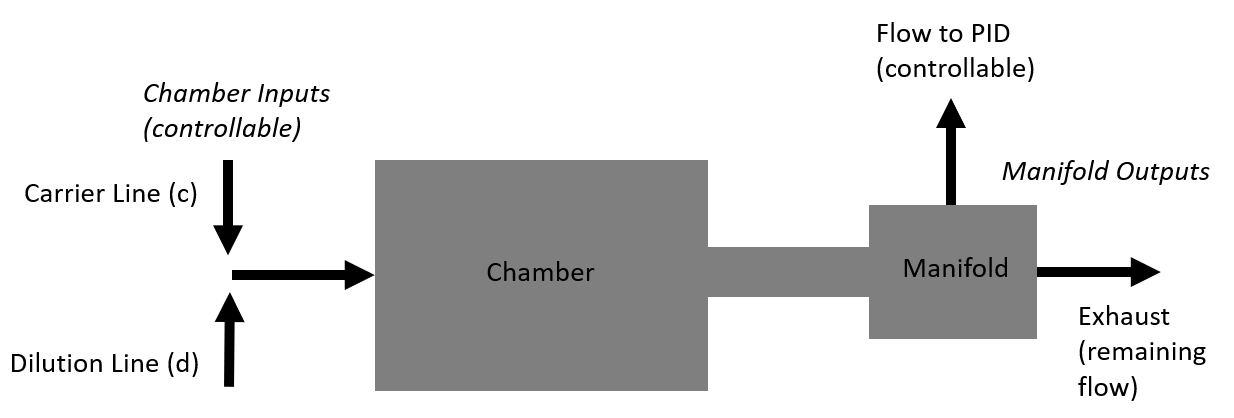
\includegraphics[width=0.9\textwidth,height=\textheight]{figures/ch5/chamber-manifold.png}

}

\caption{Vapour Delivery System - Schematic of device chamber and
manifold}

\end{figure}

\hypertarget{temperature-and-humidity-indicator}{%
\subsubsection{Temperature and Humidity
Indicator}\label{temperature-and-humidity-indicator}}

\hypertarget{photoionisation-detector}{%
\subsubsection{Photoionisation
Detector}\label{photoionisation-detector}}

\hypertarget{bubbling-vapour}{%
\paragraph*{Bubbling Vapour}\label{bubbling-vapour}}
\addcontentsline{toc}{paragraph}{Bubbling Vapour}

First year report: ``\,````First, a 200 sccm flow of N2 gas was sent
through the dilution line to the device chamber until 1000 s. Then, the
flow controller three-way valves were manually adjusted so that the same
200 sccm flow was directed through 50 mL of EtOH analyte in the carrier
line. This continued until 2200 s, where the valves were again manually
adjusted so that 200 sccm clean N2 again flowed through the device
chamber. The resulting current across the device channel was monitored
over this time, and is shown in Figure 19. A response to EtOH exposure
and removal is visible.''``\,''

\hypertarget{summary}{%
\subsection{Summary}\label{summary}}



\end{document}
